%% Copyright 2022 Boris Shminke
%%
%% Licensed under the Apache License, Version 2.0 (the "License");
%% you may not use this file except in compliance with the License.
%% You may obtain a copy of the License at
%%
%%     https://www.apache.org/licenses/LICENSE-2.0
%%
%% Unless required by applicable law or agreed to in writing, software
%% distributed under the License is distributed on an "AS IS" BASIS,
%% WITHOUT WARRANTIES OR CONDITIONS OF ANY KIND, either express or implied.
%% See the License for the specific language governing permissions and
%% limitations under the License.
\documentclass{beamer}
\usetheme{Antibes}
\usepackage{hyperref}
\usepackage{caption}
\title{Python client for Isabelle server}
\author{Boris Shminke}
\institute{Université Côte d’Azur, CNRS, LJAD, France}
\date{21 Sep 2022}
\begin{document}
\begin{frame}
\titlepage
\end{frame}
\begin{frame}
\frametitle{Motivation: Isabelle GUI is great, but}
\begin{columns}[T]
\begin{column}{0.3\textwidth}
\begin{itemize}
\item manual input
\item interactive
\item no other programming language needed
\end{itemize}
\end{column}
\begin{column}{0.7\textwidth}
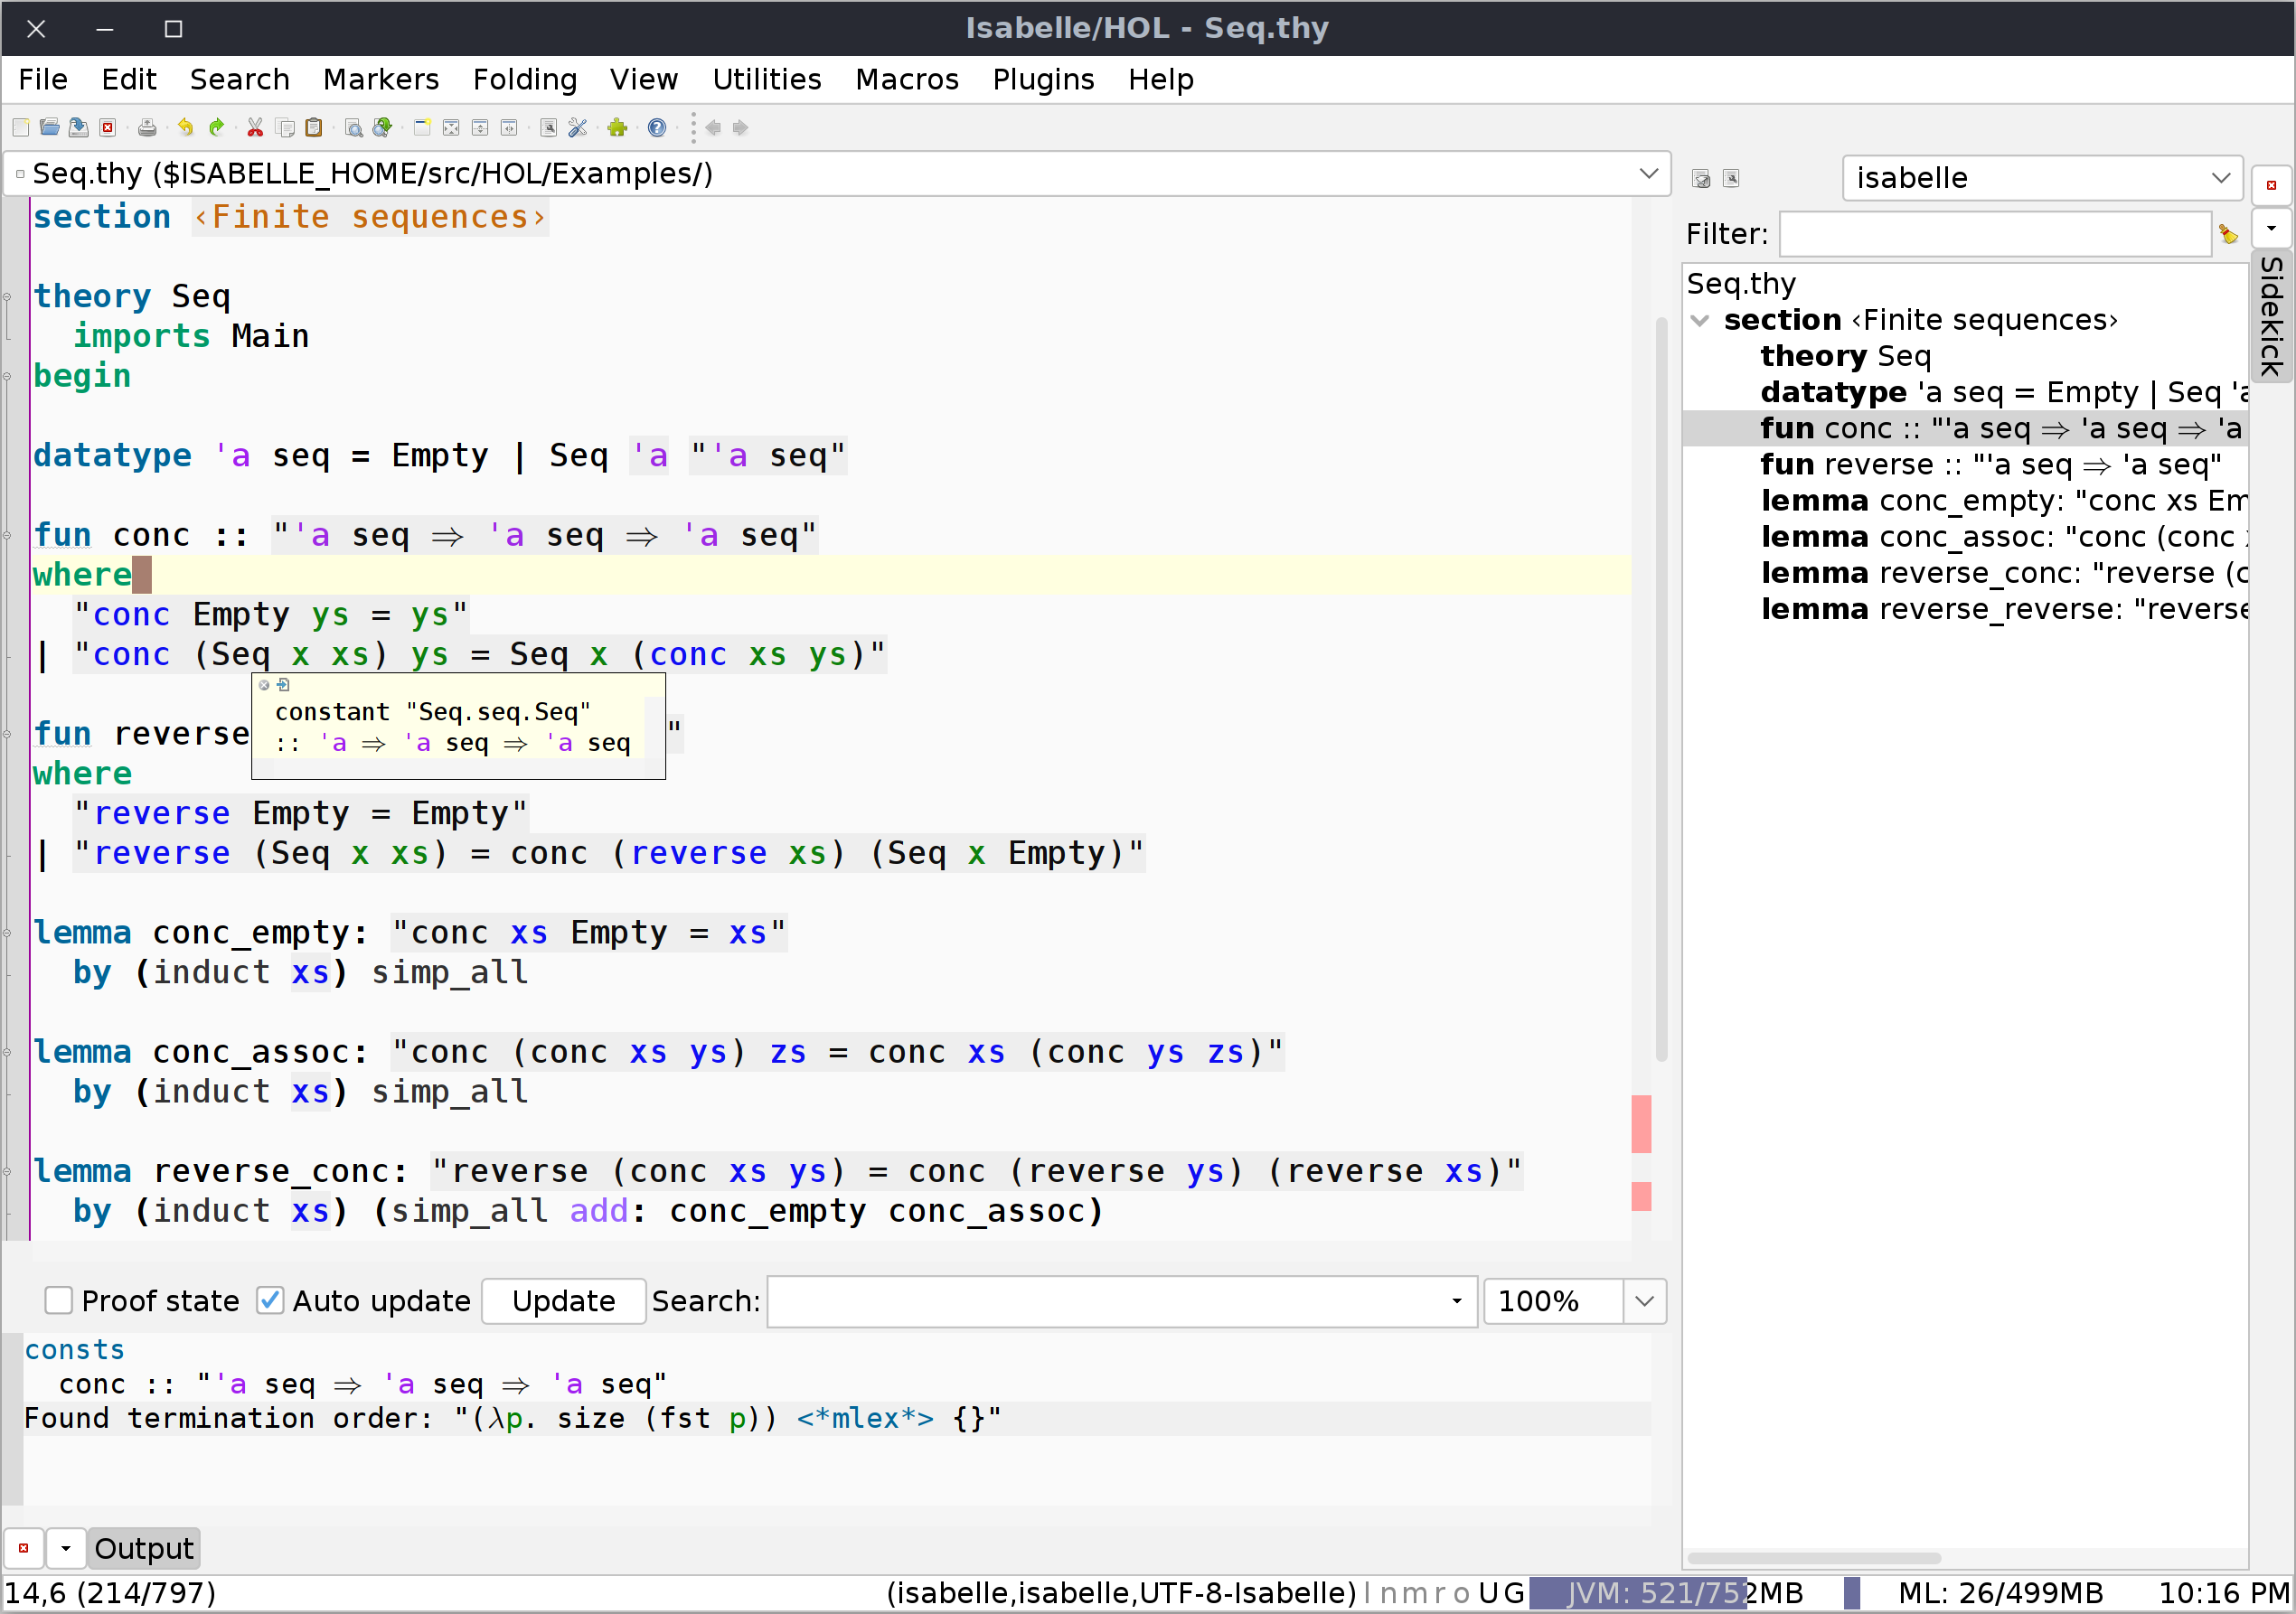
\includegraphics[width=\paperwidth,height=\paperheight]{isabelle_jedit}
\end{column}
\end{columns}
\end{frame}
\begin{frame}
\frametitle{Motivation: hacking Isabelle is demanding}
\begin{columns}[T]
\begin{column}{0.45\textwidth}
\begin{itemize}
\item input: files, streams, etc
\item one can program (nearly) anything
\item \texttt{Scala} and/or \texttt{Poly/ML}
\end{itemize}
\end{column}
\begin{column}{0.55\textwidth}
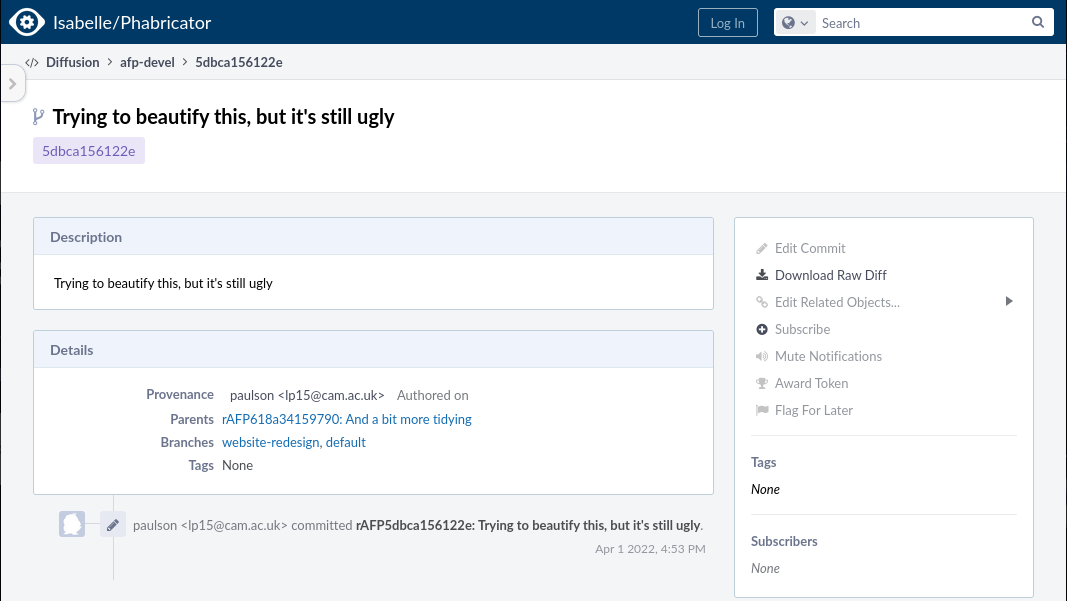
\includegraphics[width=\paperwidth,height=\paperheight]{still-ugly}
\end{column}
\end{columns}
\end{frame}
\begin{frame}[t]
\frametitle{Motivation: Isabelle server - in between}
\begin{itemize}
\item a ready solution (since 2018)
\item working with theory files (in bulk)
\item any language (through TCP)
\end{itemize}
\end{frame}
\begin{frame}
\frametitle{Demo: Isabelle server from Python}
\begin{figure}
\caption*{\url{https://bit.ly/3RnIm7v}}

\includegraphics[scale=0.25]{bit.ly_3RnIm7v.png}
\end{figure}
\end{frame}
\begin{frame}[t]
\frametitle{Demo: main takeaways}
\begin{itemize}
\item we worked with Isabelle theories as texts
\item we haven't use any language except Python
\item Isabelle did for us what it does best
\end{itemize}
\end{frame}
\begin{frame}[t]
\frametitle{What else I can do with Python client: research}
\begin{itemize}
\item generate hundreds of theories to check
\item parse \texttt{Nitpick} replies to get finite models
\item crack a research problem which stood open for two years!
\item \url{https://github.com/inpefess/residuated-binars}
\item \url{https://arxiv.org/abs/2109.05264}
\end{itemize}
\end{frame}
\begin{frame}[t]
\frametitle{What else I can do with Python client: education}
\begin{itemize}
\item teach students who know Python a bit of Isabelle syntax
\item generate finite models for different algebraic structures
\item double-check the models found in Python
\item (Advanced Logic course at the Université Côte d'Azur)
\end{itemize}
\end{frame}
\begin{frame}[t]
\frametitle{Who uses the Python client?}
\begin{itemize}
\item unfortunately, mostly its author
\item but the students from my course did
\item and Fabian Huch tested Proving for Fun backend with it
\item Haslbeck, Maximilian PL, and Simon Wimmer. Competitive Proving for Fun. Kalpa Publications in Computing 10 (2019): 9-14.
\end{itemize}
\end{frame}
\begin{frame}[t]
\frametitle{How to get the Python client?}
\begin{itemize}
\item \texttt{pip}, \texttt{conda} or \texttt{Docker}
\item Linux and Windows
\item read the docs: \url{https://isabelle-client.rtfd.io}
\end{itemize}
\end{frame}
\begin{frame}[t]
\frametitle{Future plans}
\begin{itemize}
\item continue maintaining the package
\item take part in Isabelle server development
\item hear suggestions from you!
\end{itemize}
\end{frame}
\begin{frame}[t]
\frametitle{Thank you for your attention!}
\begin{itemize}
\item happy to answer your questions now
\item or later during CICM in person
\item or by email \url{mailto:boris.shminke@univ-cotedazur.fr}
\end{itemize}
\end{frame}
\end{document}
